%
\documentclass[12pt]{article}

%% make references and citations clickable
\usepackage[backref,colorlinks=true, linkcolor=blue, citecolor=blue, urlcolor=blue, pdfborder={0 0 0}]{hyperref}

%% set the paper geometry
\usepackage[left=1in,top=1in,right=1in,bottom=1in,letterpaper]{geometry}

%% this is for arrows with text over them  --- currently not installed
%%\usepackage{mathtools}

%% uncomment the next line if you need to present an algorithm
%\usepackage{algorithm,algorithmic}

% This section is added by me (Geoff)
%-----------------------------------------------
%% standard AMS stuff
\usepackage{amssymb,amsmath,amsthm}

%% some proof-writing environments
\newenvironment{claim}[1]{\par\noindent\underline{Claim:}\space#1}{}
\newenvironment{claimproof}[1]{\par\noindent\underline{Proof:}\space#1}{}
%\newenvironment{proof}{\paragraph{Proof:}}{\hfill}
\theoremstyle{definition}
\newtheorem{theorem}{Theorem}[section]
\newtheorem{ex}[theorem]{Example}
\newtheorem{defn}[theorem]{Definition}
\newtheorem{lemma}[theorem]{Lemma}
\newtheorem{notn}[theorem]{Notation}

%% norm and abs val and inner prod
\newcommand{\norm}[1]{\left\lVert#1\right\rVert}
\newcommand{\abs}[1]{\left\lvert#1\right\rvert}
\newcommand{\iprod}[1]{\langle #1 \rangle}
\newcommand{\spn}[0]{\text{span}}

%% ceiling and floor   --- Not working for some reason
%%\DeclarePairedDelimiter\ceil{\lceil}{\rceil}
%%\DeclarePairedDelimiter\floor{\lfloor}{\rfloor}

%% kernel and image  -- Currently did something wrong
%%\newcommand{\ker}[1]{\text{ker}\left(#1\right)}
%%\newcommand{\Im}[1]{\text{Im}\left(#1\right)}  %% TODO: FIX THIS

%% Important letters/symbols
\newcommand{\ep}[0]{\epsilon}
\newcommand{\R}[0]{\mathbb{R}}
\newcommand{\bR}[0]{\bar{\mathbb{R}}}
\newcommand{\cC}[0]{\mathcal{C}}
\newcommand{\cP}[0]{\mathcal{P}}
\newcommand{\pd}[0]{\partial}

%% I had some issues with alignment, here was one online soln
%%\usepackage[fleqn]{amsmath}
%% It DIDN'T WORK THOUGH

%------------------------------------------------


%% for including urls by \url{url text}
\usepackage{url}

\newtheorem*{assumptions*}{Assumptions}
\newtheorem*{algorithm*}{Algorithm}
\usepackage{graphicx}

\begin{document}

\title{Meeting Notes 11/8/2016}
\author{Geoffrey Iyer}
\maketitle

I spent a lot of time this week thinking about what assumptions we should make about our data set, and what our classification goals should be. For now, I'm working entirely theoretically. I haven't yet thought about how to make this computationally feasible. Here's what I came up with in the end.

\subsection*{Assumptions}
We have two data sets, $X_1,X_2$, both sampling the same underlying scene. There exists a bijective correpondence $X_1 \to X_2$ based on how the data was sampled. For example: we could have $X_1,X_2$ are both timeseries images of the same scene, taken from different angles. In this case the correspondence would be based on the time the image was taken.

I also assume that we have already determined some number of correspondence pairs $m$, where $m < < \abs{X}$. I notated these as $\{p_1,\ldots,p_m\} \subseteq X_1$ and $\{q_1,\ldots,q_m\}\subseteq X_2$.

Lastly, I assume that the data sets $X_1, X_2$ have somehow been normalized so that distances between points are roughly comparable between sets.

\subsection*{Goal}
With these assumptions, I believe we can construct a latent space $X$ and mappings $X_1, X_2 \to X$ that allow us to extract information from the combined data that we could not get from either individual set. In particular, we are interested in differences between two data points that can be seen through one set, but not the other.

\subsection*{Algorithm}
\begin{enumerate}
\item First, we attempt to reconstruct the full point correspondence between $X_1,X_2$ using the distinguished pairs
  $\{p_j\}\subseteq X_1$ and $\{q_j\}\subseteq X_2$.
Let $\rho : X_1\to X_2$ be a bijection that preserves our distinguished pairs $\{p_j\}, \{q_j\}$. We'll define an energy $E(\rho)$ that we can minimize to find the optimal bijection. For notation, let
\[X_1 - \{p_1,\ldots,p_m\} = \{x_1,\ldots,x_n\}.\]
Then define the energy
\[E(\rho) = \sum_{i=1}^m\sum_{j=1}^n \max\left( \norm{p_i-x_j}, \norm{q_i -\rho(x_j)}\right).\]
I'm honestly not too confident about this choice for $E$. It seems like it will give reasonable results, but it's hard to say if this is the best (especially compared to using $+$ over $\max$). The idea here is that when we sample from our source to obtain $X_j$, we lose some information. So if two elements are close together in $X_j$, that doesn't necessarily mean that they are close in the original sample. However, if points are far apart in $X_j$, then they should be considered far apart in the original sample.

If we somehow find a $\rho$ that minimizes the above energy, we proceed to step 2.

\item Now we have constructed a full correspondence $\rho$ we move on to the creation of our latent space $X$. Our goal is to embed $X_1, X_2$ into $X$ while preserving
  \[\max\left( \norm{x_i - x_j}, \norm{\rho(x_i) - \rho(x_j)}\right).\]
  That is, if our points are considered close together in $X_1$, and far apart in $X_2$, they should be thought of as far apart in our latent space $X$. I didn't get very far in my experiment with this, but it seems like we should be able to do this by mimicking the idea from \cite{Wang11}. Knowing the correspondence pairs let's us put extra weight in our Graph Laplacian towards keeping those points together.
\end{enumerate}

\subsection*{Toy Example}
This section is going to be rushed. I didn't have time to make my examples look nice. Here are pictures of the ground truth data (figure \ref{img:ground-truth}), $X_1$ (figure \ref{img:X_1}), and $X_2$ (figure \ref{img:X_2}). The ground truth contains 3 gaussian clouds (with 3 points each). $X_1$ and $X_2$ are the projections onto the $xy$ and $xz$ planes (respectively).

For starting assumptions, I picked a one point from each cloud to be a known correspondence pair (so the $m$ above is 3. One from each cloud). I think minimized the energy from step 1 by explicitely calculating it for each permutation (so $6!$ total calculations). It usually did okay, but rarely over got the exact correct correspondence from the ground truth. Sounds like I need to rework my idea.

For step 2, I assumed that I already had the correct correspondence from the ground truth (since step 1 wasn't working too well). Then I followed the idea from \cite{Wang11} and built a weight matrix that tracked when points were known to correspond (I called it $W_s$). As well as the standard graph laplacian on each individual $X_j$ (I called the concatenated matrix $W$). Constructing the corresponding graph laplacian $L + L_s$ and doing the standard eignvector analysis yielded okay results. It mostly clusted the 3 clouds together, but usually there were some strange outliers. So it's certainly not a perfect method but there was some promise.

\begin{figure}
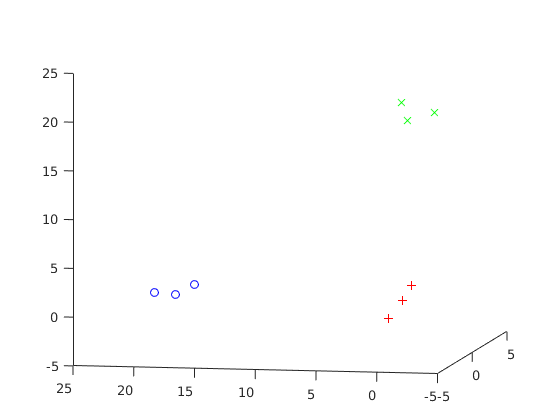
\includegraphics[width=\linewidth]{Ground_Truth.png}
\caption{Ground Truth}
\label{img:ground-truth}
\end{figure}

\begin{figure}
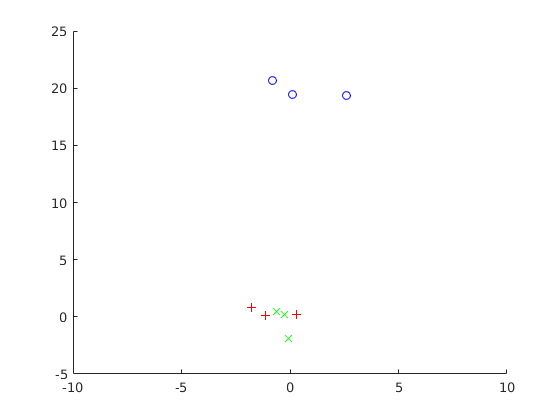
\includegraphics[width=\linewidth]{X_1.png}
\caption{$X_1$}
\label{img:X_1}
\end{figure}

\begin{figure}
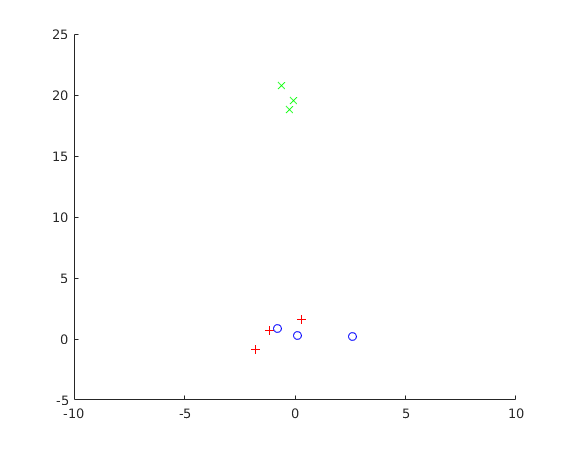
\includegraphics[width=\linewidth]{X_2.png}
\caption{$X_2$}
\label{img:X_2}
\end{figure}

\bibliographystyle{plain}
\bibliography{../../BibTex/research}
\end{document}
